\chapter{Bifurcations of fixed points}
\section{Local nonlinear dynamics near fixed points}
We are interested in the local nonlinear dynamics around fixed points. Consider
\begin{align}
	\dot{x}=f(x);\quad f\in C^{r},r \geq 1; \quad f(p) = 0, \numberthis \label{eq:4star}
\end{align}
i.e. $p$ is a fixed point of the dynamical system. The linearized system at $p$ is
\begin{align}
	\dot{y} = Df(p)y,\ y\in \mathbb{R}^{n},\ Df(p)\in \mathbb{R}^{n \times n}. \numberthis \label{eq:4sstar}
\end{align}
The linearization has the eigenvalues $\lambda_1, \ldots, \lambda_n \in \mathbb{C}$ with multiplicities counted. Corresponding to these eigenvalues are the eigenvectors $e_1,\ldots,e_n \in \mathbb{C}^{n}$, including generalized eigenvectors for when the algebraic multiplicity is greater than the geometric multiplicity. The eigenvector $e_j$ is real when $\lambda_j \in \mathbb{R}$.

\begin{definition}
The following subspaces are invariant for the linearized dynamical system:
\begin{enumerate}
	\item The \emph{stable subspace}
		\begin{align}
			\boxed{
				E^{S} =  \textrm{span} _{j}\left \{  \textrm{Re} (e_j),  \textrm{Im} (e_j):\  \textrm{Re} (e_j) < 0\right\},
			}
		\end{align}
	\item The \emph{unstable subspace}
		\begin{align}
			\boxed{
				E^{U} =  \textrm{span} _{j}\left \{  \textrm{Re} (e_j),  \textrm{Im} (e_j):\  \textrm{Re} (e_j) > 0\right\},
			}
		\end{align}
	\item The \emph{center subspace}
		\begin{align}
			\boxed{
				E^{C} =  \textrm{span} _{j}\left \{  \textrm{Re} (e_j),  \textrm{Im} (e_j):\  \textrm{Re} (e_j) = 0\right\}.
			}
		\end{align}
\end{enumerate}

\end{definition}
\begin{remark}[]
	Note here that the following facts hold
	\begin{enumerate}
		\item $E^{C}= \emptyset$ if and only if $p$ is hyperbolic,
		\item $E^{U,S}$ and $E^{C}$ are invariant subspaces of \eqref{eq:4sstar} by construction,
		\item Solutions of \eqref{eq:4sstar} in $E^{S}$ (resp. $E^{U}$) decay to $y=0$ as $t \to \infty$ (resp. $t \to - \infty$). 
	\end{enumerate}
	
\end{remark}

We now ask ourselves what happens to these subspaces in the nonlinear system.
\begin{theorem}[Center Manifold Theorem]
	The following hold:
	\begin{enumerate}
		\item There exists a unique \emph{stable manifold} $W^{S}(p)$ for \eqref{eq:4star}, such that
	\begin{itemize}
		\item $W^{S}(p)$ is a $C^{r}$ manifold (surface), tangent to $E^{S}$ at $p$ with $ \textrm{dim} W^{S}(p) =  \textrm{dim} E^{S}$,
		\item $W^{S}(p)$ is invariant for \eqref{eq:4star} and for $x\in W^{S}(p)$ we have 
			\begin{align}
				\| F^{t}(x) \| \leq K_{S} \exp\left[ t \left( \max_{ \textrm{Re} (\lambda_j) < 0}( \textrm{Re} (\lambda_j)) + \epsilon_S \right) \right]
			\end{align}
	 for $t\geq 0$, $0 < \epsilon_S \ll 1$, and  $\| x- p\|$ small enough.
	\end{itemize}
			
		\item There exists a unique \emph{unstable manifold} $W^{U}(p)$ for \eqref{eq:4star}, such that
	\begin{itemize}
		\item $W^{U}(p)$ is a $C^{r}$ manifold (surface), tangent to $E^{U}$ at $p$ with $ \textrm{dim} W^{U}(p) =  \textrm{dim} E^{U}$,
		\item $W^{U}(p)$ is invariant for \eqref{eq:4star} and for $x\in W^{U}(p)$ we have 
			\begin{align}
				\| F^{t}(x) \| \leq K_{U} \exp\left[ t \left( \max_{ \textrm{Re} (\lambda_j) > 0}( \textrm{Re} (\lambda_j)) + \epsilon_U \right) \right]
			\end{align}
	 for $t\geq 0$, $0 < \epsilon_U \ll 1$, and  $\| x- p\|$ small enough.
	\end{itemize}
			
\item There exists a (not necessarily unique) \emph{center manifold} $W^{C}(p)$ for \eqref{eq:4star}, such that
	\begin{itemize}
		\item $W^{C}(p)$ is a $C^{r-1}$ manifold (surface), tangent to $E^{C}$ at $p$ with $ \textrm{dim} W^{C}(p) =  \textrm{dim} E^{C}$,
	\end{itemize}
			
	\end{enumerate}
	
\end{theorem}
The geometry of these manifolds is sketched in Fig. \ref{fig:mfds_def}.
\begin{figure}[h!]
	\centering
	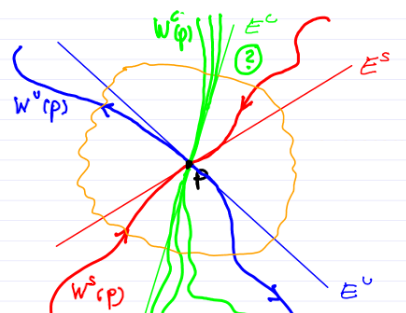
\includegraphics[width=0.6\textwidth]{figures/ch3/1manifolds_def.png}
	\caption{A sketch of the stable (red), unstable (blue), and center manifolds (green), along with their respective invariant linear subspaces. Note the existence of multiple center manifolds and the singular unique unstable/stable manifolds.}
	\label{fig:mfds_def}
\end{figure}

The overall dynamics depend crucially on the center manifold, especially when $E^{U}= \emptyset$, i.e. the stability type is determined by $W^{C}(p)$. Hence why it will be the subject of our further investigation.

\section{The center manifold}
\begin{ex}[Uniqueness of the center manifold]
	We would like to explore if the center manifold is generally non-unique. Consider the dynamical system
	\begin{align}
\begin{dcases}
	\dot{x} = x^2 \\
	\dot{y} = -y.
\end{dcases}
	\end{align}
	First, linearize at the origin to find the linearized dynamics
	\begin{align}
		A = Df(0) = 
		\begin{pmatrix}
			0 & 0 \\ 0 & -1
		\end{pmatrix}
		.
	\end{align}
	These linearized dynamics are illustrated in Fig. \ref{fig:cmfd_lin_ex}. We find the invariant subspaces
	\begin{align}
		E^{C} =  \textrm{span}\left\{ 
			\begin{pmatrix}
				1 \\ 0 
			\end{pmatrix}
		\right\};\quad
		E^{S} =  \textrm{span}  \left\{
			\begin{pmatrix}
				0 \\ 1
			\end{pmatrix}
		\right\}; \quad
		E^{U} = \emptyset.
	\end{align}
	The nonlinear manifolds are illustrated with the invariant subspaces from the linearization in Fig. \ref{fig:cmfd_lin_ex}.
	\begin{figure}[h!]
		\centering
		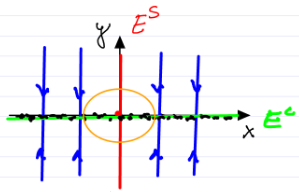
\includegraphics[width=0.45\textwidth]{figures/ch3/2cmfd_lin_ex.png}
		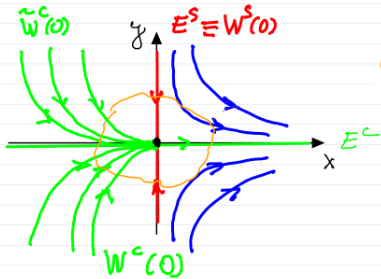
\includegraphics[width=0.4\textwidth]{figures/ch3/3cmfd_nonlin_ex.png}
		\caption{Left: The linearized dynamics around the origin. Right: The nonlinear phase portrait. }
		\label{fig:cmfd_lin_ex}
	\end{figure}
	Observe there exist infinitely many center manifolds which are all invariant and all tangent to $E^{C}$ at the origin. We also see that although the fixed point at the origin is stable in the linearized system, it is unstable in the nonlinear system.
\end{ex}

We are left with the question: how can we calculate $W^{C}(p)$ in general? 
\begin{enumerate}
	\item Consider 
		\begin{align}
			\dot{z} = F(z); \quad F(0) = 0;\quad z \in \mathbb{R}^{c+d};\quad F \in C^{r}.
		\end{align}
		Where $c$ represents the number of center directions at the origin ($ \textrm{dim}E^{C}$) and $d$ denoted the remaining directions ($ \textrm{dim} E^{U} +  \textrm{dim} E^{S}$).
	\item Now block-diagonalize the linearization. This consists of four steps
		\begin{enumerate}
			\item First linearize the dynamics to find $\dot{z} = Mz + \mathcal{O}(\|z\|^2)$ with $M = DF(0) \in \mathbb{R}^{(c+d) \times (c+d)}$.
			\item Define the transformation matrix
				\begin{align}
					T=
					\begin{bmatrix}
						a_1 & \ldots & a_c & b_1 & \ldots & b_d	
					\end{bmatrix}
				=
				\begin{bmatrix}
					\textrm{basis in } E^{C} &  \textrm{basis in } E^{U} \oplus E^{S}
				\end{bmatrix}
				.
				\end{align}
			\item Pass to the basis from the transformation matrix with $z = T \xi$
				\begin{align}
					\dot{\xi} = T^{-1}\dot{z} = T^{-1}MT \xi + T^{-1}\mathcal{O}(\| T\xi\|^2) = 
					\begin{pmatrix}
						A & 0 \\
						0 & B
					\end{pmatrix}
					\xi + \mathcal{O}(\| \xi \| ^2).
				\end{align}
			The matrices $A$ and $B$ are elements of $\mathbb{R}^{c \times c}$ and $\mathbb{R}^{d \times d}$ respectively.	
		\item Let $\xi = 
			\begin{pmatrix}
				x \\ y
			\end{pmatrix}
			\in \mathbb{R}^{c}\times \mathbb{R}^{d}$, the $x$-coordinates is aligned with $E^{C}$ and the $y$-coordinates are perpendicular. We then find
			\begin{align}
				\dot{x} = Ax + f(x,y);\quad \dot{y} = By + g(x,y),
			\end{align}
			for $f,g \in C^{r}$ and $f,g = \mathcal{O}(\|x\|^2, \|y\|^2, \|x\|\|y\|)$. The geometry in these coordinates is depicted in Fig. \ref{fig:cmfd_trafo_geom}. The center manifold is given by
			\begin{align}
				W^{C}(0) = \left\{ (x,y) \in U:\ y = h(x)\right\}
			\end{align}
			for $h:\mathbb{R}^{c} \to \mathbb{R}^{d}$ and $ h \in C^{r-1}$ as in the theorem.
			\begin{figure}[h!]
				\centering
				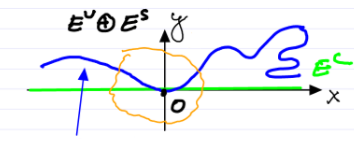
\includegraphics[width=0.4\textwidth]{figures/ch3/4cmfd_trafo_geom.png}
				\caption{The geometry of the nonlinear system in the transformed coordinates aligned with the invariant subspaces of the linearization. The blue arrow points to the center manifold $W^{C}(0)$.}
				\label{fig:cmfd_trafo_geom}
			\end{figure}
		\end{enumerate}
	\item Now we use the invariance of $W^{C}(0)$, i.e. for all $t$ it holds $y(t) = h(x(t))$ to find
		\begin{align}
			\dot{y} = Dh(x(t)) \dot{x}(t),
		\end{align}
		which implies the nonlinear partial differential equation (PDE) for $h(x)$
\begin{align}
	\boxed{
		Bh(x) + g(x, h(x)) = Dh(x) \left[ Ax + f(x, h(x))\right] \numberthis \label{eq4:1star}.
	}
\end{align}
We cannot solve this analytically.
\item Instead take the Taylor expansion of \eqref{eq4:1star} to approximate the solution
	\begin{align}
		h(x) = \underbrace{h(0)}_{=0} + \underbrace{Dh(0)}_{=0}x + \frac{1}{2} \underbrace{D^2h(0)}_{3- \textrm{tensor} } \otimes x \otimes x + \mathcal{O}(\|x \| ^3),
	\end{align}
	where the first two terms are 0 due to the tangency to $E^{C}$ at $0$. We therefore have that $h(x) = \mathcal{O}(\|x\|^2)$. Therefore we seek $W^{C}(0)$ of this form. We get the dynamics on the center manifolds 
	\begin{align}
		\boxed{
			\dot{x}=Ax+f(x,h(x)).
		}
	\end{align}
\end{enumerate}

\begin{ex}[Finding the center manifold]
	Consider the dynamical system
	\begin{align}
		\begin{dcases}
			\dot{x}=xy \\
			\dot{y}=-y+\alpha x.
		\end{dcases}	
	\end{align}
	First we linearize at $(0,0)$ to get 
	\begin{align}
		M =
		\begin{pmatrix}
			[0] & [0] \\
			[0] & [-1]
		\end{pmatrix}
	\end{align}
	which is already in block-matrix form. The dimensions of the stable, unstable, and center subspaces of the linearization are 1, 0, and 1 respectively. Hence the stability type depends on the dynamics on the center manifold $W^{C}(0)$. We now look for an equation to parameterize $W^{C}(0)$
	\begin{align}
		h(x) = ax^2 + bx^3 + cx^4 + \mathcal{O}(x^5).
	\end{align}
	This is a finite expansion and thus in general will not converge as that would imply the center manifold is unique. Now use the invariance (the PDE we already derived) to find
	\begin{align}
		\dot{y} = h'(x)\dot{x} = \left[2ax+3bx^2 + 4cx^3 + \mathcal{O}(x^4) \right] x \left[ax^2+bx^3+cx^4 + \mathcal{O}(x^5) \right]. \numberthis \label{eq4:one}	
	\end{align}
	On the other hand, from the dynamical system we know
	\begin{align}
		\dot{y}=-h(x) + \alpha x^2 =(\alpha - a) x^2 -bx^3 - cx^4 + \mathcal{O}(x^5). \numberthis \label{eq4:two}
	\end{align}
	Comparing coefficients of equal powers in \eqref{eq4:one} and \eqref{eq4:two}.
	\begin{align}
		\mathcal{O}(x^2)&:\ \alpha = a\\
		\mathcal{O}(x^3)&:\ b=0 \\
		\mathcal{O}(x^4)&:\ 2a^2 = -c.
	\end{align}
	Therefore we find 
	\begin{align}
		\boxed{
	h(x) =\alpha x^2 - 2\alpha^2x^4 + \mathcal{O}(x^5).}
	\end{align}
	Then the dynamics on $W^{C}(0)$ become
	\begin{align}
		\boxed{
			\dot{x}= xh(x) = \alpha x^3(1-2\alpha x^2) + \mathcal{O}(x^6). \numberthis \label{eq4:2star}
		}
	\end{align}
	These dynamics are depicted in Fig. \ref{fig:cmfd_alpha_diff}. For $\alpha > 0$ the origin is unstable, meanwhile for $ \alpha <0$ the origin is asymptotically stable.
	\begin{figure}[h!]
		\centering
		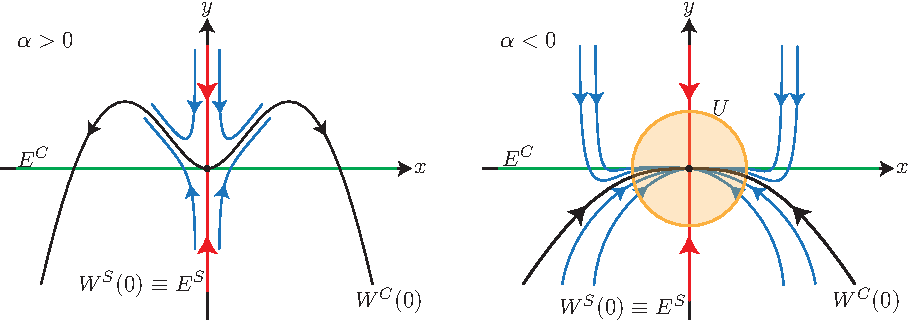
\includegraphics[width=0.8\textwidth]{figures/ch3/5cmfd_alpha_diff}
		\caption{Left: The nonlinear dynamics on the center manifold for $\alpha > 0$. Right: The nonlinear dynamics on the center manifold for $\alpha < 0$.}
		\label{fig:}
	\end{figure}
	
	The full local stable manifold for $\alpha <0$ is $\overline{W}^{S}(0)=U$ and it is of dimension 2. The difference between $\overline{W}^{S}(0)$ and $W^{S}(0)$ is that in general the decay rate is generally weaker than the rate guaranteed in the Center Manifold Theorem. 

\begin{remark}[]
	The $\mathcal{O}(x^5)$ truncation has two hyperbolic fixed points at $x = \pm \frac{1}{\sqrt{2 \alpha} }$, however the full system has no such fixed points. The reason for this is that away from the origin, the $\mathcal{O}(x^6)$ terms are no longer guaranteed to be small relative to the $\mathcal{O}(x^5)$ terms, and the truncation this far away from 0 is not justified.
\end{remark}
\end{ex}

After this example we would like to explore if the concept of the center manifold is robust, as the existence of eigenvalues with $ \textrm{Re} (\lambda_i) = 0$ is not.
